\section{Data-driven results for the 2D SWE}\label{sec:data-driven-results-2D}
In this section we will present the results for the 2D SWE using the data-driven models.
We consider the same initial condition (Gaussian function) as in the 1D case, but now in two dimensions.
We solve the 2d SWE using both a CNN and a FNO model, and compare the results in terms of run time and accuracy.
We also compare the run time to the numerical method FVM, to see if the data-driven models can be used as a faster alternative to the FVM.
We also test the ability of the FNO model to generalize to a finer grid, by training the model on a coarse grid and then making predictions on a fine grid.
Finally, we will test the FNO model's ability to generalize further in time and make long-term predictions.


\subsection{2D SWE with initial Gaussian function}
The initial condition for the 2D problem is a Gaussian function with a standard deviation of 0.1 and a mean of 0.5.
The initial condition can be seen in \autoref{fig:2D_gauss_initial_condition}.
\begin{figure}[H]
    \centering
    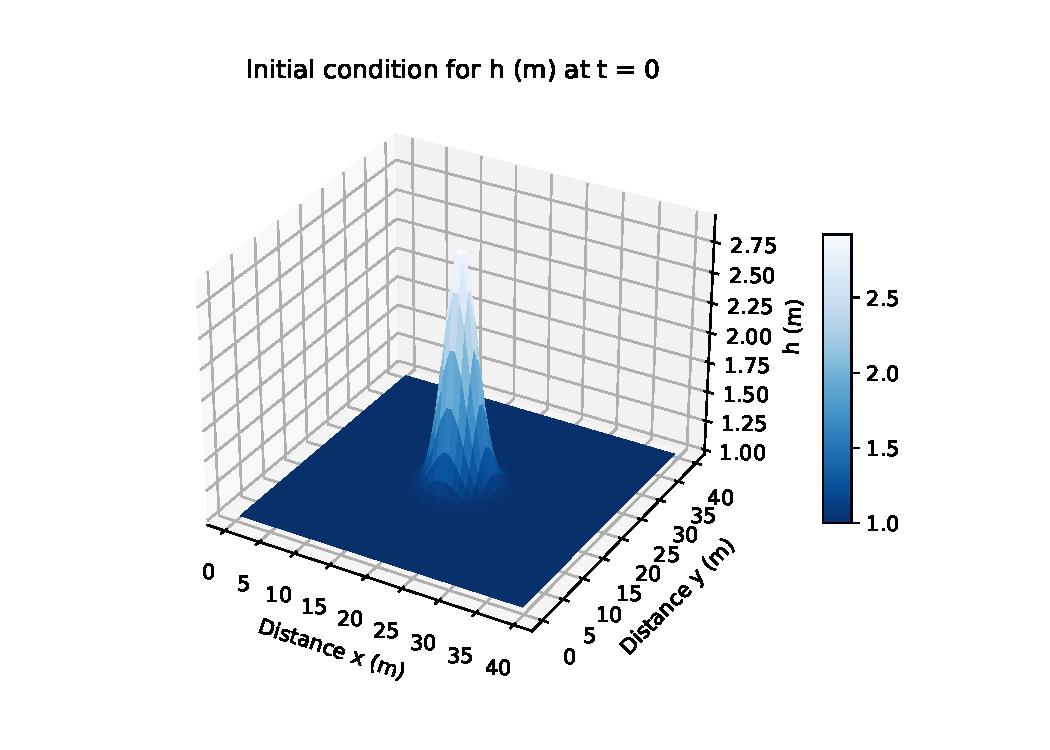
\includegraphics[width=0.8\textwidth]{C:/Users/Matteo/Shallow-Water-Equations/plots/2D_gauss_initial_condition.pdf}
    \caption{Initial condition for the 2D problem.}\label{fig:2D_gauss_initial_condition}
\end{figure}
\subsubsection*{CNN Model}


The training and validation loss for the 2D CNN model can be seen in \autoref{fig:2D_CNN_loss}.
\begin{figure}[H]
    \centering
    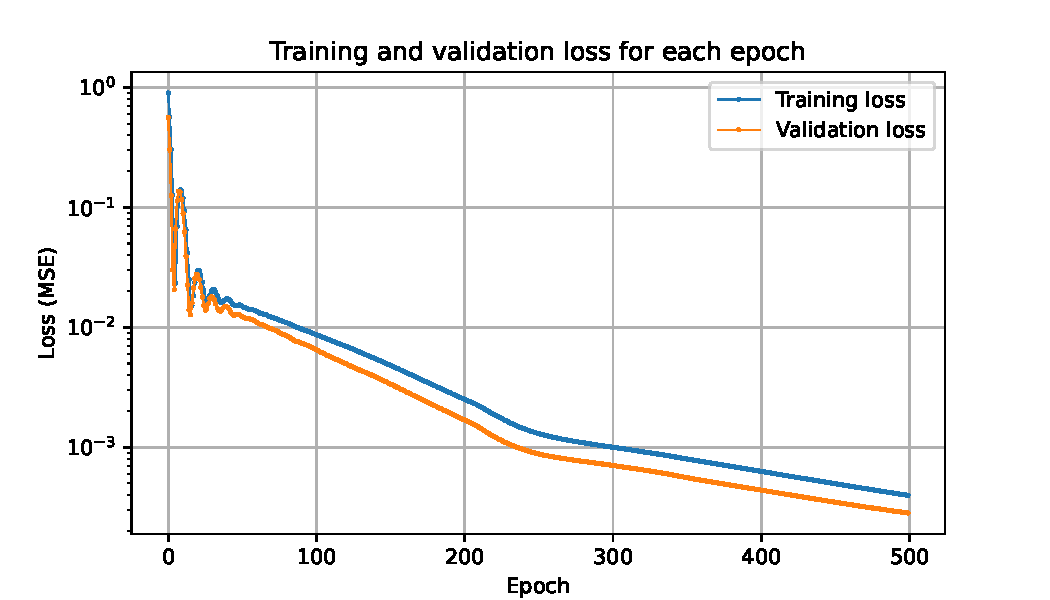
\includegraphics[width=0.7\textwidth]{C:/Users/Matteo/Shallow-Water-Equations/plots/2D_CNN_loss.pdf}
    \caption{Training and validation loss for the 2D CNN model.}\label{fig:2D_CNN_loss}
\end{figure}

The error plot for the last prediction for the 2D CNN can be seen in \autoref{fig:2D_CNN_error}.
\begin{figure}[H]
    \centering
    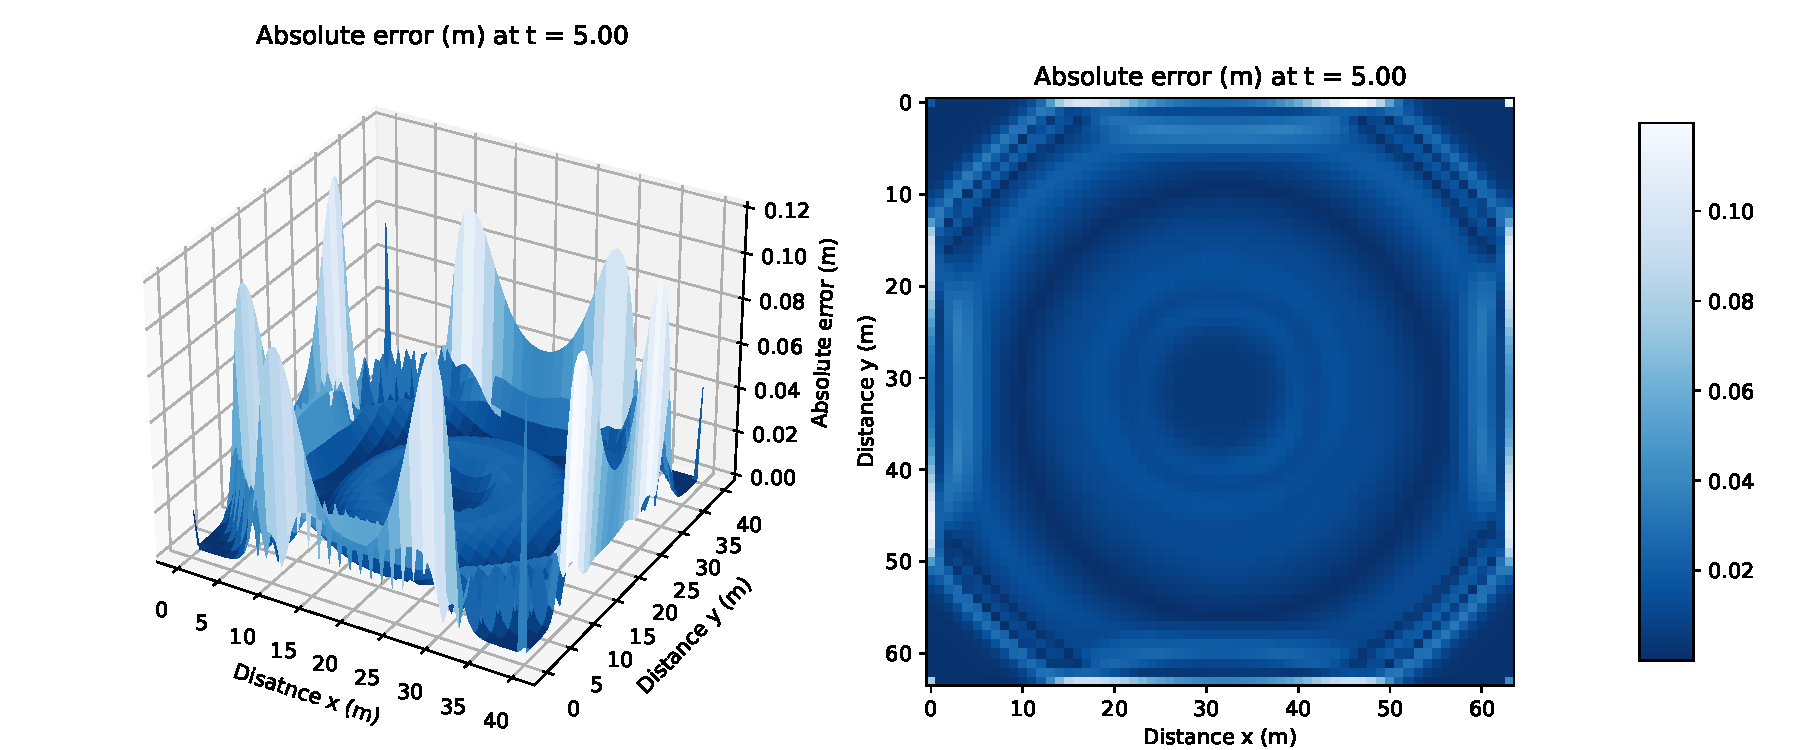
\includegraphics[width=0.8\textwidth]{C:/Users/Matteo/Shallow-Water-Equations/plots/2D_CNN_error.pdf}
    \caption{Error plot for the last prediction for the 2D CNN.}\label{fig:2D_CNN_error}
\end{figure}

\subsubsection*{FNO Model}
The training and validation loss for the 2D FNO model can be seen in \autoref{fig:2D_FNO_loss}.
\begin{figure}[H]
    \centering
    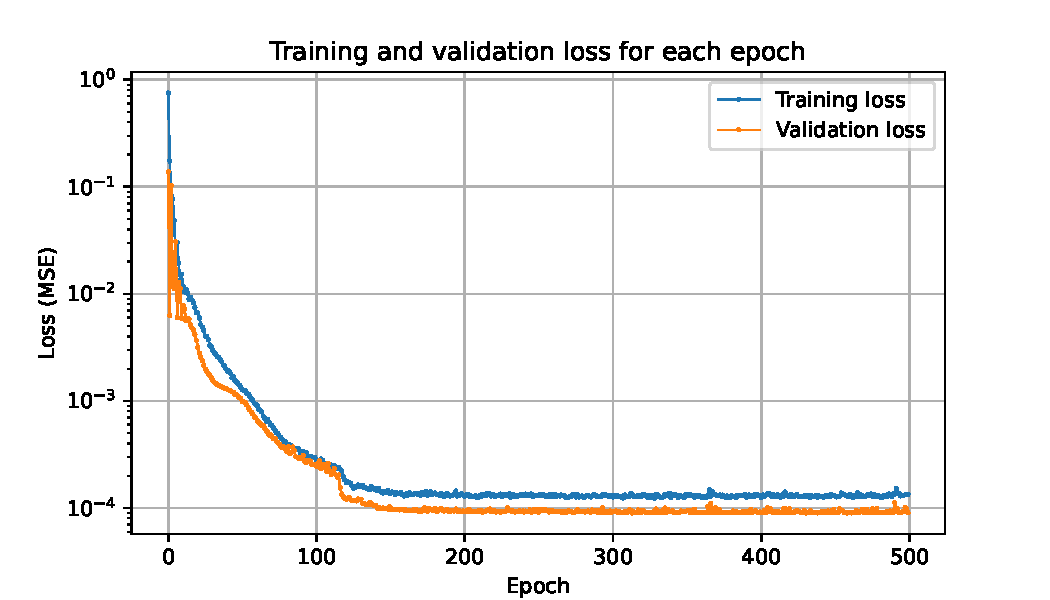
\includegraphics[width=0.8\textwidth]{C:/Users/Matteo/Shallow-Water-Equations/plots/2D_FNO_loss.pdf}
    \caption{Training and validation loss for the 2D FNO model.}\label{fig:2D_FNO_loss}
\end{figure}

The error plot for the last prediction for the 2D FNO can be seen in \autoref{fig:2D_FNO_error}.
\begin{figure}[H]
    \centering
    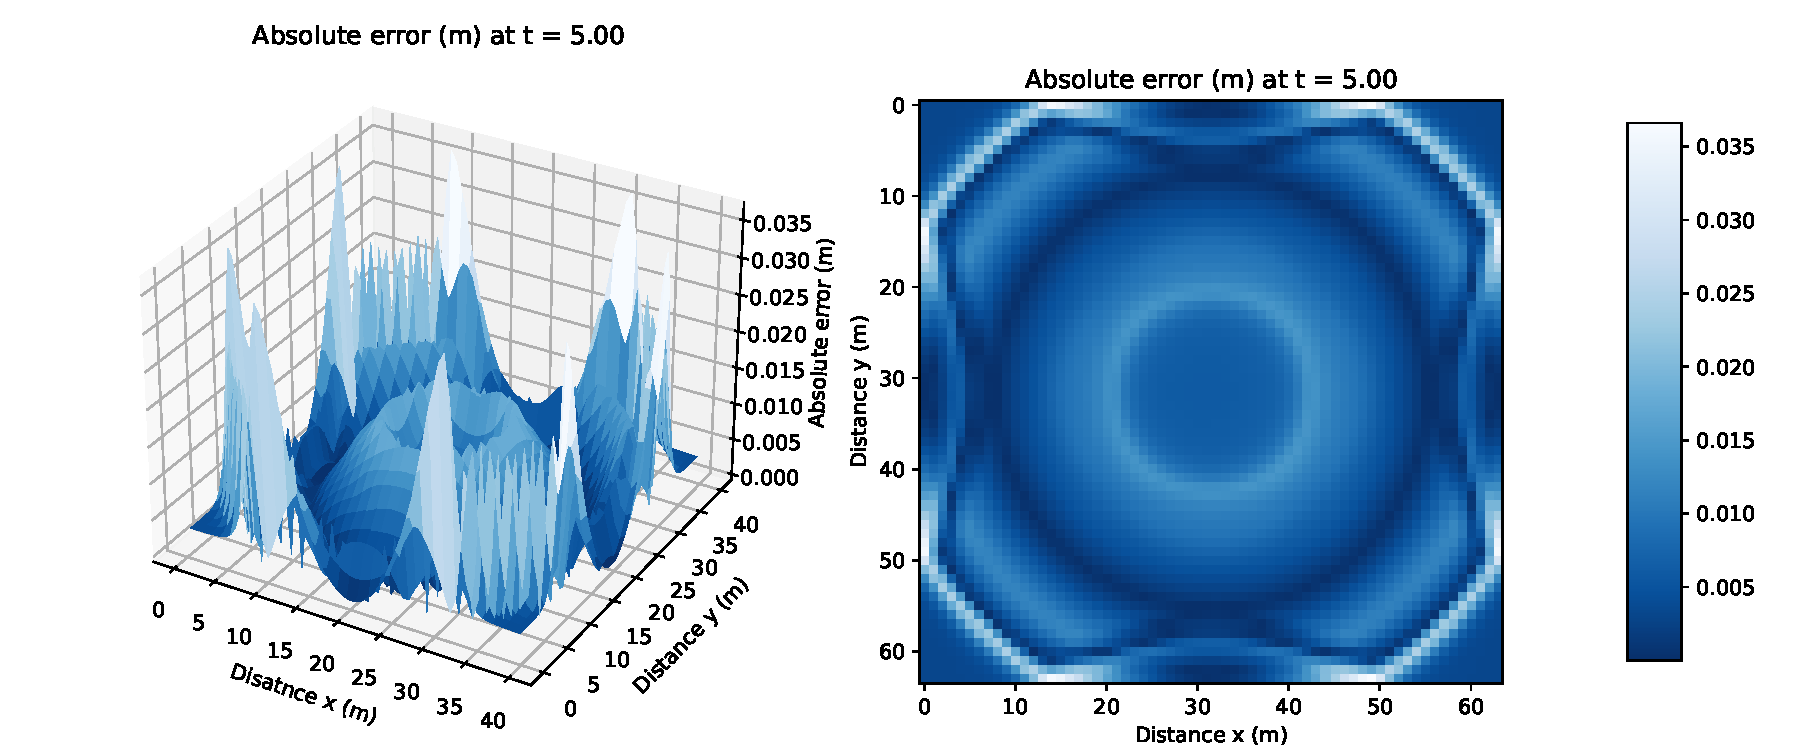
\includegraphics[width=0.8\textwidth]{C:/Users/Matteo/Shallow-Water-Equations/plots/2D_FNO_error.pdf}
    \caption{Error plot for the last prediction for the 2D FNO.}\label{fig:2D_FNO_error}
\end{figure}


\subsubsection*{Comparison}
To get an overview of the performance of the different models, we consider the MSE and MAE for the predictions for the 2D SWE case.
\begin{table}[H]
    \centering
    \small % Reduce font size
    \begin{tabular}{c|cccc|cccc}
        Model & \multicolumn{4}{c|}{$N = 64$} & \multicolumn{4}{c}{$N = 128$} \\
        \cline{2-9}
        & Epochs & MSE & MAE & Time (s) & Epochs & MSE & MAE & Time (s) \\
        \hline
        CNN  &
        \input{C:/Users/Matteo/Shallow-Water-Equations/saved_results/2D_CNN_Nx=64_nepochs.txt} &
        \input{C:/Users/Matteo/Shallow-Water-Equations/saved_results/2D_CNN_Nx=64_MSE_test.txt} & 
        \input{C:/Users/Matteo/Shallow-Water-Equations/saved_results/2D_CNN_Nx=64_MAE_test.txt} &
        \input{C:/Users/Matteo/Shallow-Water-Equations/saved_results/2D_CNN_Nx=64_time.txt} &
        \input{C:/Users/Matteo/Shallow-Water-Equations/saved_results/2D_CNN_Nx=128_nepochs.txt} &
        \input{C:/Users/Matteo/Shallow-Water-Equations/saved_results/2D_CNN_Nx=128_MSE_test.txt} &
        \input{C:/Users/Matteo/Shallow-Water-Equations/saved_results/2D_CNN_Nx=128_MAE_test.txt} &
        \input{C:/Users/Matteo/Shallow-Water-Equations/saved_results/2D_CNN_Nx=128_time.txt} 
        \\
        \hline
        FNO  &
        \input{C:/Users/Matteo/Shallow-Water-Equations/saved_results/2D_FNO_Nx=64_nepochs.txt} &
        \input{C:/Users/Matteo/Shallow-Water-Equations/saved_results/2D_FNO_Nx=64_MSE_test.txt} &
        \input{C:/Users/Matteo/Shallow-Water-Equations/saved_results/2D_FNO_Nx=64_MAE_test.txt} &
        \input{C:/Users/Matteo/Shallow-Water-Equations/saved_results/2D_FNO_Nx=64_time.txt} &
        \input{C:/Users/Matteo/Shallow-Water-Equations/saved_results/2D_CNN_Nx=128_nepochs.txt} &
        \input{C:/Users/Matteo/Shallow-Water-Equations/saved_results/2D_FNO_Nx=128_MSE_test.txt} &
        \input{C:/Users/Matteo/Shallow-Water-Equations/saved_results/2D_FNO_Nx=128_MAE_test.txt} &
        \input{C:/Users/Matteo/Shallow-Water-Equations/saved_results/2D_FNO_Nx=128_time.txt}
        \\
        \hline
    \end{tabular}
    \caption{Test loss in terms of MSE and MAE, and time for training the models for the 2D SWE.}\label{tab:results_2D_comparison}
\end{table}
We see that the FNO model in general needs fewer epochs to converge compared to the CNN model, but it also takes longer time to train.
From the theory we know that FNO are supposed to work when we are training on a coarse grid and then make predictions on a fine grid.
To test this, we will train the models on a coarse grid and then make predictions on a fine grid.
The table below shows the results when the FNO-model is trained on a grid with $N = 64$ and then makes predictions on a grid with $N = 128$.
\begin{table}[H]
    \centering
    \begin{tabular}{c|ccc}
        Model & \multicolumn{3}{c}{$N = 128$} \\
        \cline{2-4}
        & MSE & MAE & Prediction time (s) \\
        \hline
        FNO  &
        \input{C:/Users/Matteo/Shallow-Water-Equations/saved_results/2D_FNO_train_Nx=64_test_N=128_MSE_test.txt} &
        \input{C:/Users/Matteo/Shallow-Water-Equations/saved_results/2D_FNO_train_Nx=64_test_N=128_MAE_test.txt} &
        \input{C:/Users/Matteo/Shallow-Water-Equations/saved_results/2D_FNO_train_Nx=64_test_N=128_time.txt}
    \end{tabular}
    \caption{Test loss in terms of MSE and MAE, and time for training the FNO model on a grid with $N = 64$ and then making predictions on a grid with $N = 128$.}\label{tab:results_2D_FNO_train_64_test_128}
\end{table}
From the results in \autoref{tab:results_2D_FNO_train_64_test_128} we see that the FNO model is able to generalize to a finer grid.
This way, it is possible to train the model on a coarse grid and then make predictions on a fine grid, which is a great advantage when solving the SWE numerically, as it is very computationally expensive to solve the SWE on a fine grid using the FVM.

We will also time the predictions to compare the speed of the models.
We can also compare to the run time of the numerical method FVM, see \autoref{tab:scalability}.
Handle the scalability isssues.
\begin{table}[H]
    \centering
    \small % Reduce font size
    \begin{tabular}{c|ccccc}
        Model & \multicolumn{5}{c}{$N = 256$} \\
        \cline{2-6}
        & Epochs & MSE & MAE & Training time (s) & Prediction time (s) \\
        \hline
        CNN & 
        & & & & \\
        \hline
        FNO &
        & & & & \\
        \hline
    \end{tabular}
    \caption{Test loss in terms of MSE and MAE, and time for training the models for the 2D SWE.}\label{tab:results_2D_comparison_256}
\end{table}

We are also very interested in testing the ability of the FNO to generalize further in time.
We will therefore train the models on a time interval $[t_0, t_1]$ and make predictions for $t = 10$.

